%% -*- coding:utf-8 -*-
%%

\documentclass[submit,techreq,noauthor]{ipsj}

\input{dummy}
\def\newblock{\hskip .11em plus .33em minus .07em}

\usepackage[dvips]{graphicx}

\setcounter{巻数}{53}%vol53=2012
\setcounter{号数}{2}
\setcounter{page}{1}

\begin{document}
\title{AIITにおけるプロジェクト型学修(PBL)のためのBacklogシステムの導入}
\affiliate{AIIT}{産業技術大学院大学\\
AIIT, Shinagawa, Tokyo 140--0011, Japan}
\author{中鉢 欣秀}{Yoshihide Chubachi}{AIIT}[yc@aiit.ac.jp]
\author{小山 裕司}{Hiroshi Koyama}{AIIT}

\begin{abstract}
 産業技術大学院大学(以下,AIIT)ではPBLによる高度専門職人材の育成に取り
 組んでいる。AIITの学生はほとんどが社会人であるため,円滑なプロジェクト活
 動を支援するグループウェアなどの整備に取り組んできた.2012年度より新た
 にBacklogシステムを導入しPBLでの利用を開始した.このシステムの導入およ
 び現在までの運用において得られた知見を報告する.
\end{abstract}

\maketitle

\section{はじめに}

産業技術大学院大学(Advanced Institute of Industrial Technology)では,高
度な職業人材を育成するために必要となる学修のための情報インフラストラクチャ
を,在学生・修了生等に対して提供している
\cite{中鉢欣秀:2012-03-15, 小山裕司:2011, 石島辰太郎:2010, 中鉢欣秀:2010}
.また,実践的な業務遂行能力を育成するために,1年間のプロジェクト
型学修を必修とし,すべての学生が修士課程の2年次にプロジェクト活動を行なう
ことがカリキュラムの柱となっている\cite{加藤由花:2009, 戸沢義夫:2007-08-23}.

情報アーキテクチャ専攻では「情報システム学特別演習」を,創造技術専攻で
は「イノベーションデザイン特別演習」という科目名でPBLを開講している.合
計で20組のプロジェクトがあり,各プロジェクトには3〜8名程度の学生が所属
している.

AIITでは,これらのプロジェクト活動を支援するためのグループウェアとして
iPBL(Infrastructure for PBL)を導入し運用してきた
\cite{chubachi:2010:pbl, 中鉢欣秀:2009-05}.従来のシステムは,
Microsoft社のProject Server 2010を中心とした構成で,WBSによるプロジェク
ト管理システムとShare Point Servicesによるファイル共有機能を提供した.
しかしながら,Windows OSにおいてInternet Explorerでの利用を前提としてい
ることやユーザインタフェイスの使い勝手などについて,学生や教員から改善
要求が多く出されていた.

そこで,AIITでは2012年度春より,新たに
Backlog\footnote{http://www.backlog.jp/}をプロジェクト内でのコラボレー
ション・ツールとして導入した.初年度のため,従来のiPBLと併用する形で用
いることを想定し,全学生に利用を推奨しているわけではない.ここでは,半
年間の予備的な運用を通して,従来よりも改善された点や明らかになった課題
点などについて考察する.

\section{Backlogの導入と考察}

\subsection{Backlogについて}
Backlogはnulab社が提供するプロジェクト管理ツールである.従来のiPBLは学
内に専用サーバを設置して運用していたが,今回はASPの形態でライセンスを購
入した.AIITで利用しているBacklogのトップページを図\ref{fig:backlog}に
示す.

Backlogの主要な機能は,

\begin{enumerate}
 \item 課題管理
 \item ガントチャート
 \item ファイル共有
 \item バーンダウンチャート
\end{enumerate}

である.また,プログラミングを行うプロジェクト向けに,ソースコードのバー
ジョン管理をSubversionとGitで行えるようにした.

\begin{figure}[tb]
\begin{center}
\includegraphics[width=7.5cm]{./figure/backlog_screenshot.eps}
\end{center}
\caption{AIITにおけるBacklogの利用画面}
\label{fig:backlog}
\end{figure}

\subsection{ストレージの使用量からみる利用状況}
はじめに,ファイル共有機能の利用状況を示す.各プロジェクトごとの容量は
5GBに設定し,大きめのファイルを扱いたいときは別途ファイルストレージを準
備してもらうことにした.

\begin{figure}[tb]
\begin{center}
\includegraphics[width=7.5cm]{./figure/fig1.eps}
\end{center}
\caption{ストレージの使用量}
\label{fig:fig1}
\end{figure}

今年度前期が終わった8/31現在のBacklogのストレージの使用量を図
\ref{fig:fig1}に示す.Backlogの活用はプロジェクトごとに偏りがみられた.
1/4程度のプロジェクトはまったく未使用である.ストレージの使用量だけをみ
るとファイル共有の消費が目立ち,実際ファイル共有だけに使っているプロジェ
クトが多い.Wikiは8プロジェクトのみが使い,バージョン管理は利用開始願い
が必要であり,5プロジェクトだけがこれを使っている.

\subsection{課題アクション数の状況}

\begin{figure}[tb]
\begin{center}
\includegraphics[width=7.5cm]{./figure/fig2.eps}
\end{center}
\caption{課題アクション数}
\label{fig:fig2}
\end{figure}

図\ref{fig:fig2}に4/1から8/25までの課題アクション数をまとめた
\footnote{なお,8/11以降は夏休み期間のため活動量が少ない.}.課題アク
ション数とは新規課題の作成,コメント,作業進捗及び完了の報告の数である.
情報アーキテクチャ専攻では突出して利用しているプロジェクトと,ほとんど
未使用だと思われるプロジェクトがある等,程度の違いはあるが,すべてのプ
ロジェクトで課題管理を使っている.これに対して,創造技術専攻では4プロジェ
クトがかろうじて使っているだけであった.

\begin{figure}[tb]
\begin{center}
\includegraphics[width=7.5cm]{./figure/fig3.eps}
\end{center}
\caption{1メンバあたり課題アクション数}
\label{fig:fig3}
\end{figure}

\subsection{一人あたりの課題アクション数}
情報アーキテクチャ専攻の各プロジェクトのひとりあたりの課題アクション数
を整理したものが,図\ref{fig:fig3}である.平均すると1メンバあたり1日1件
程度のアクションである.

\begin{figure}[tb]
\begin{center}
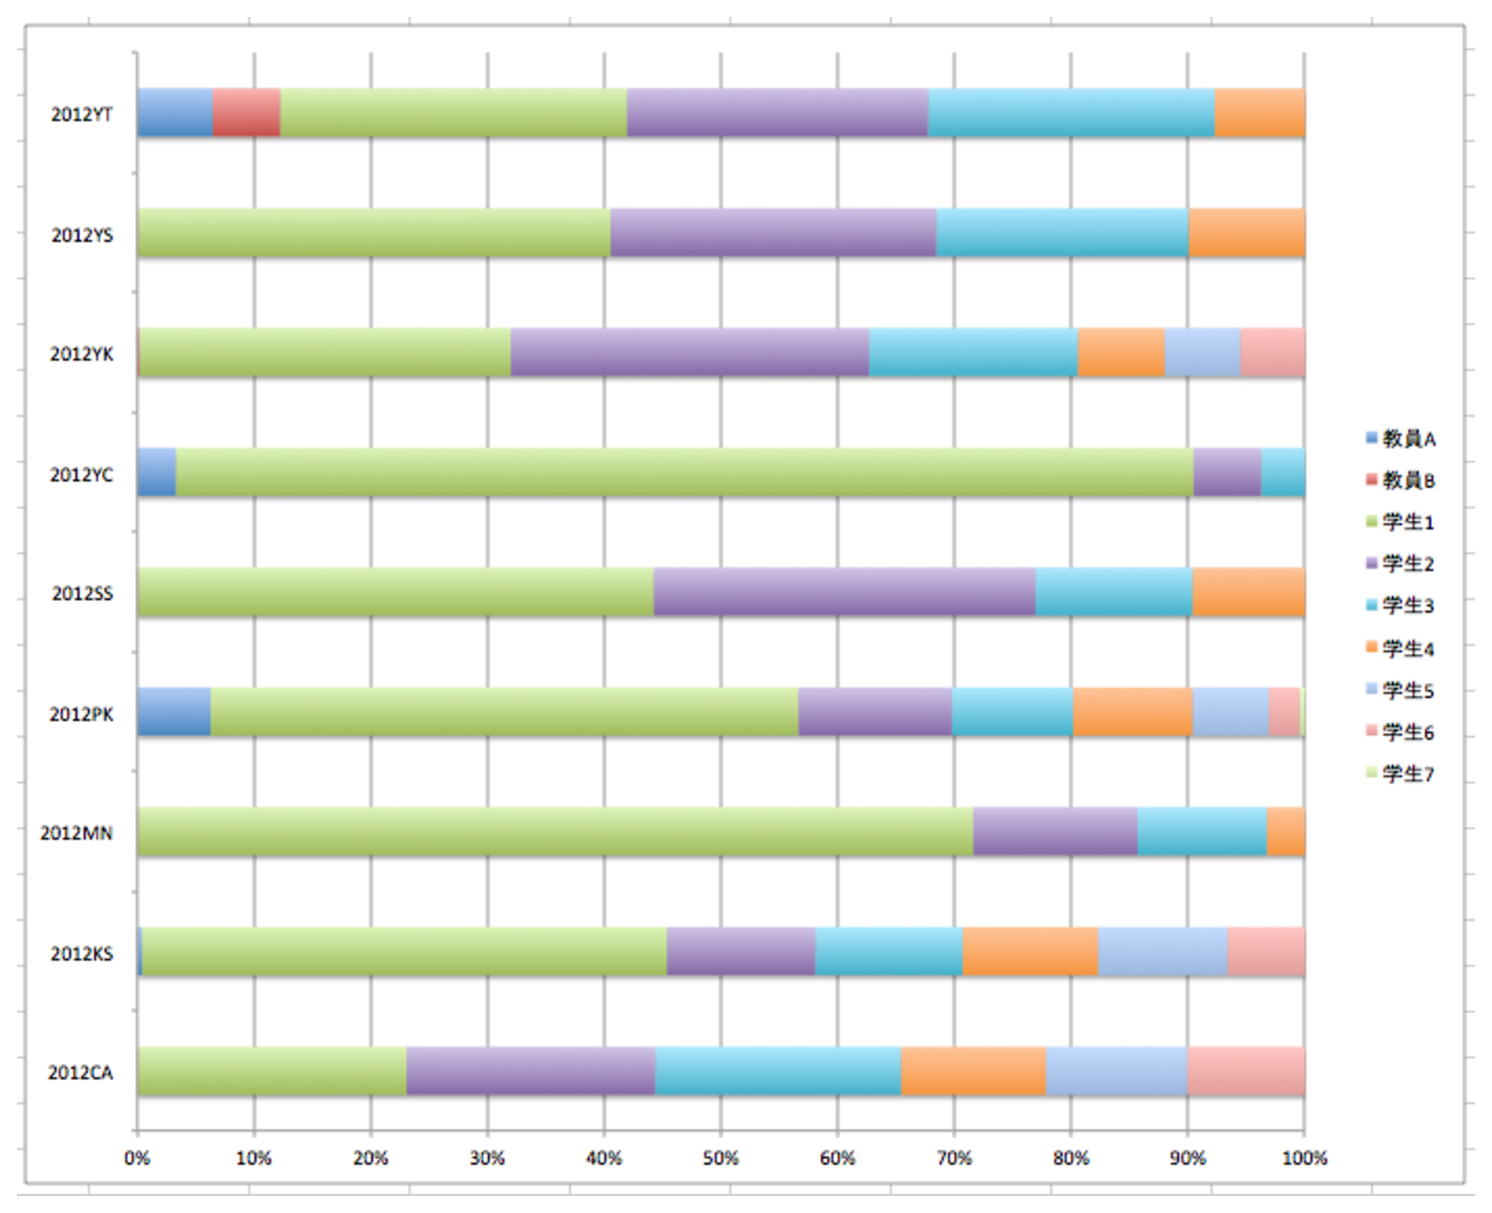
\includegraphics[width=7.5cm]{./figure/fig4.eps}
\end{center}
\caption{1メンバあたり課題アクション数}
\label{fig:fig4}
\end{figure}

これを構成メンバの関与の程度をパーセンテージで示したものが図
\ref{fig:fig4}である.メンバ内での役割の違いに依存するが,3プロジェクト
では特定の1名が50\%以上関与している状況が見られる.特に,あプロジェクト
では約87\%が特定の1名のアクションである.このように,メンバーが実施した
アクションに関するパーセンテージには,偏りがみられた.

\section{Backlog利用状況に関する考察}
ここまで見てきたとおり,現状においてはBacklogはすべてのプロジェクトで
活用できている状況ではない.これは試行的に導入しているという現状ではや
むを得ないが,ファイルの共有機能など,有効に利用されているものもあるの
で,今後はより積極的に活用するように促していく必要がある.

また,本稿で述べたとおり,Backlogの課題管理を有効に活用することで,プ
ロジェクトメンバーごとの活動の状況を定量的に示すことができる.PBLにお
けるメンバーの活動状況の見える化に有効に利用できるものと期待する.

\section{おわりに}

専門職大学院におけるPBLによる学修を支援するためのコラボレーションツール
として,Backlogを導入した事例について報告した.現状においてはプロジェク
ト毎によって活用の度合いにばらつきがある.

Backlogを用いることで,学生の作成した成果物の量や,取り組んだ課題の数を
定量化することができる.今後はこの特性を活かし,AIITにおけるPBLの教育効
果を向上させるための仕組みとして利用することを目指したい.

\bibliographystyle{junsrt}
\bibliography{bibliography/chubachi}

\appendix

参考として,Backlogの主要な機能の画面のスクリーンショットを図
\ref{fig:File}〜\ref{fig:Wiki1}までに示す.

\begin{figure}[t]
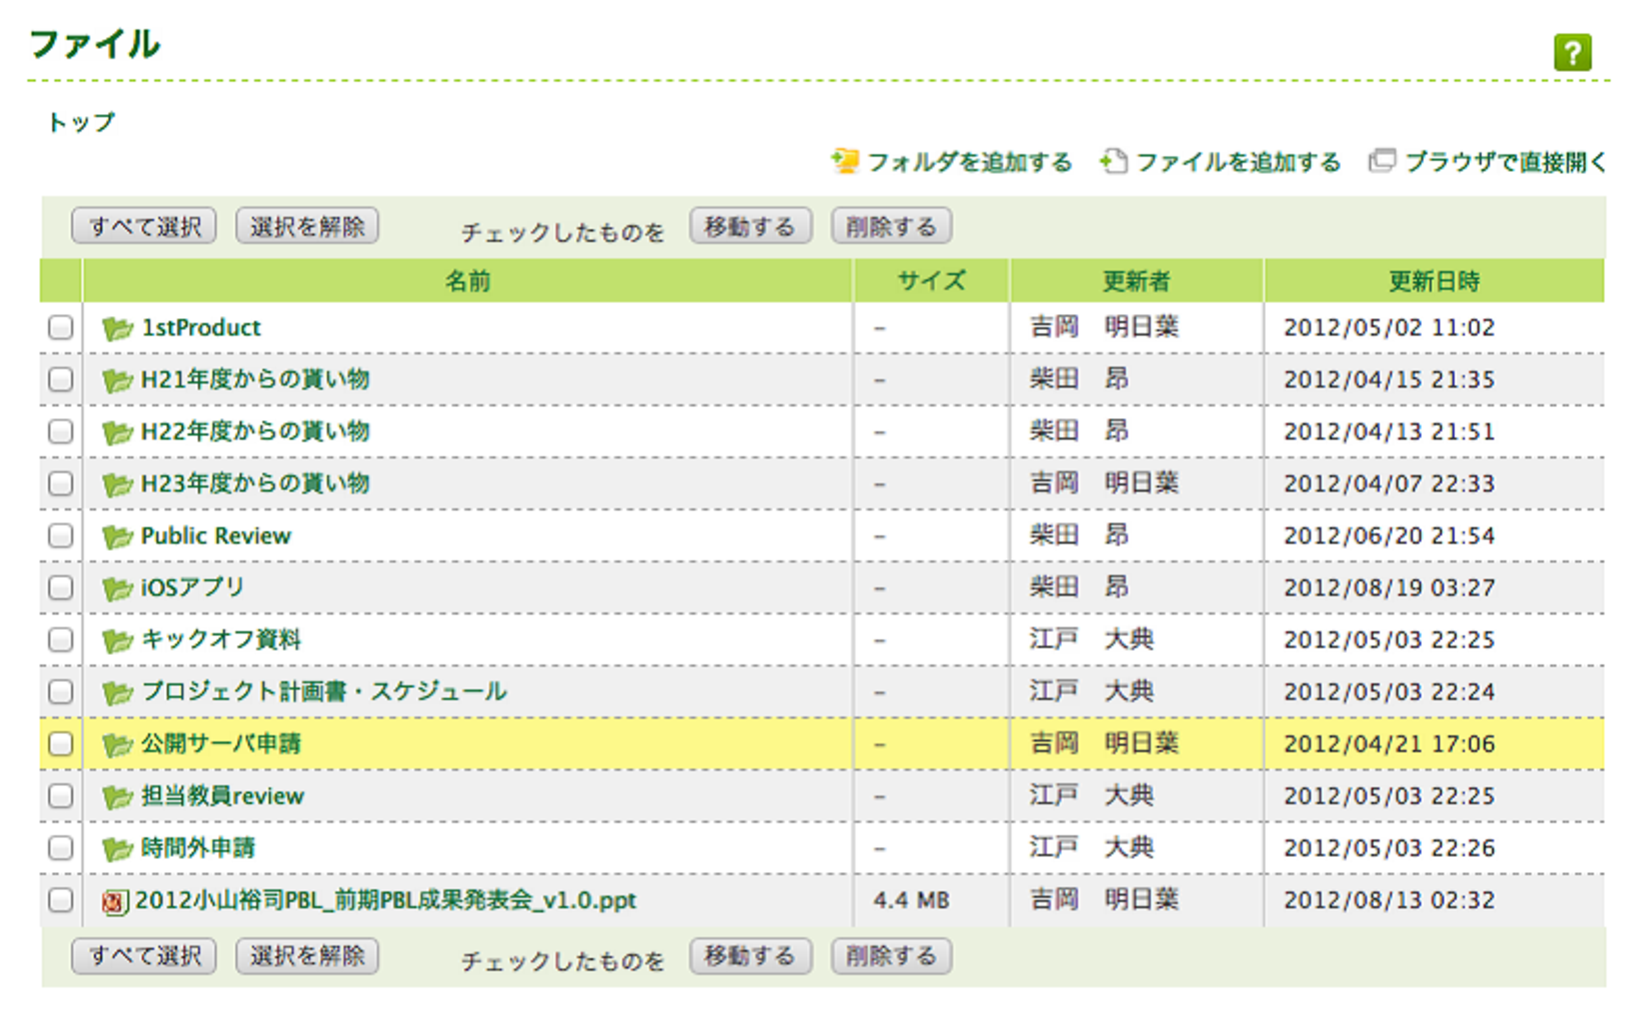
\includegraphics[width=7.5cm]{./figure/File.eps}
\caption{プロジェクトでのファイル共有}
\label{fig:File}
\end{figure}

\begin{figure}[t]
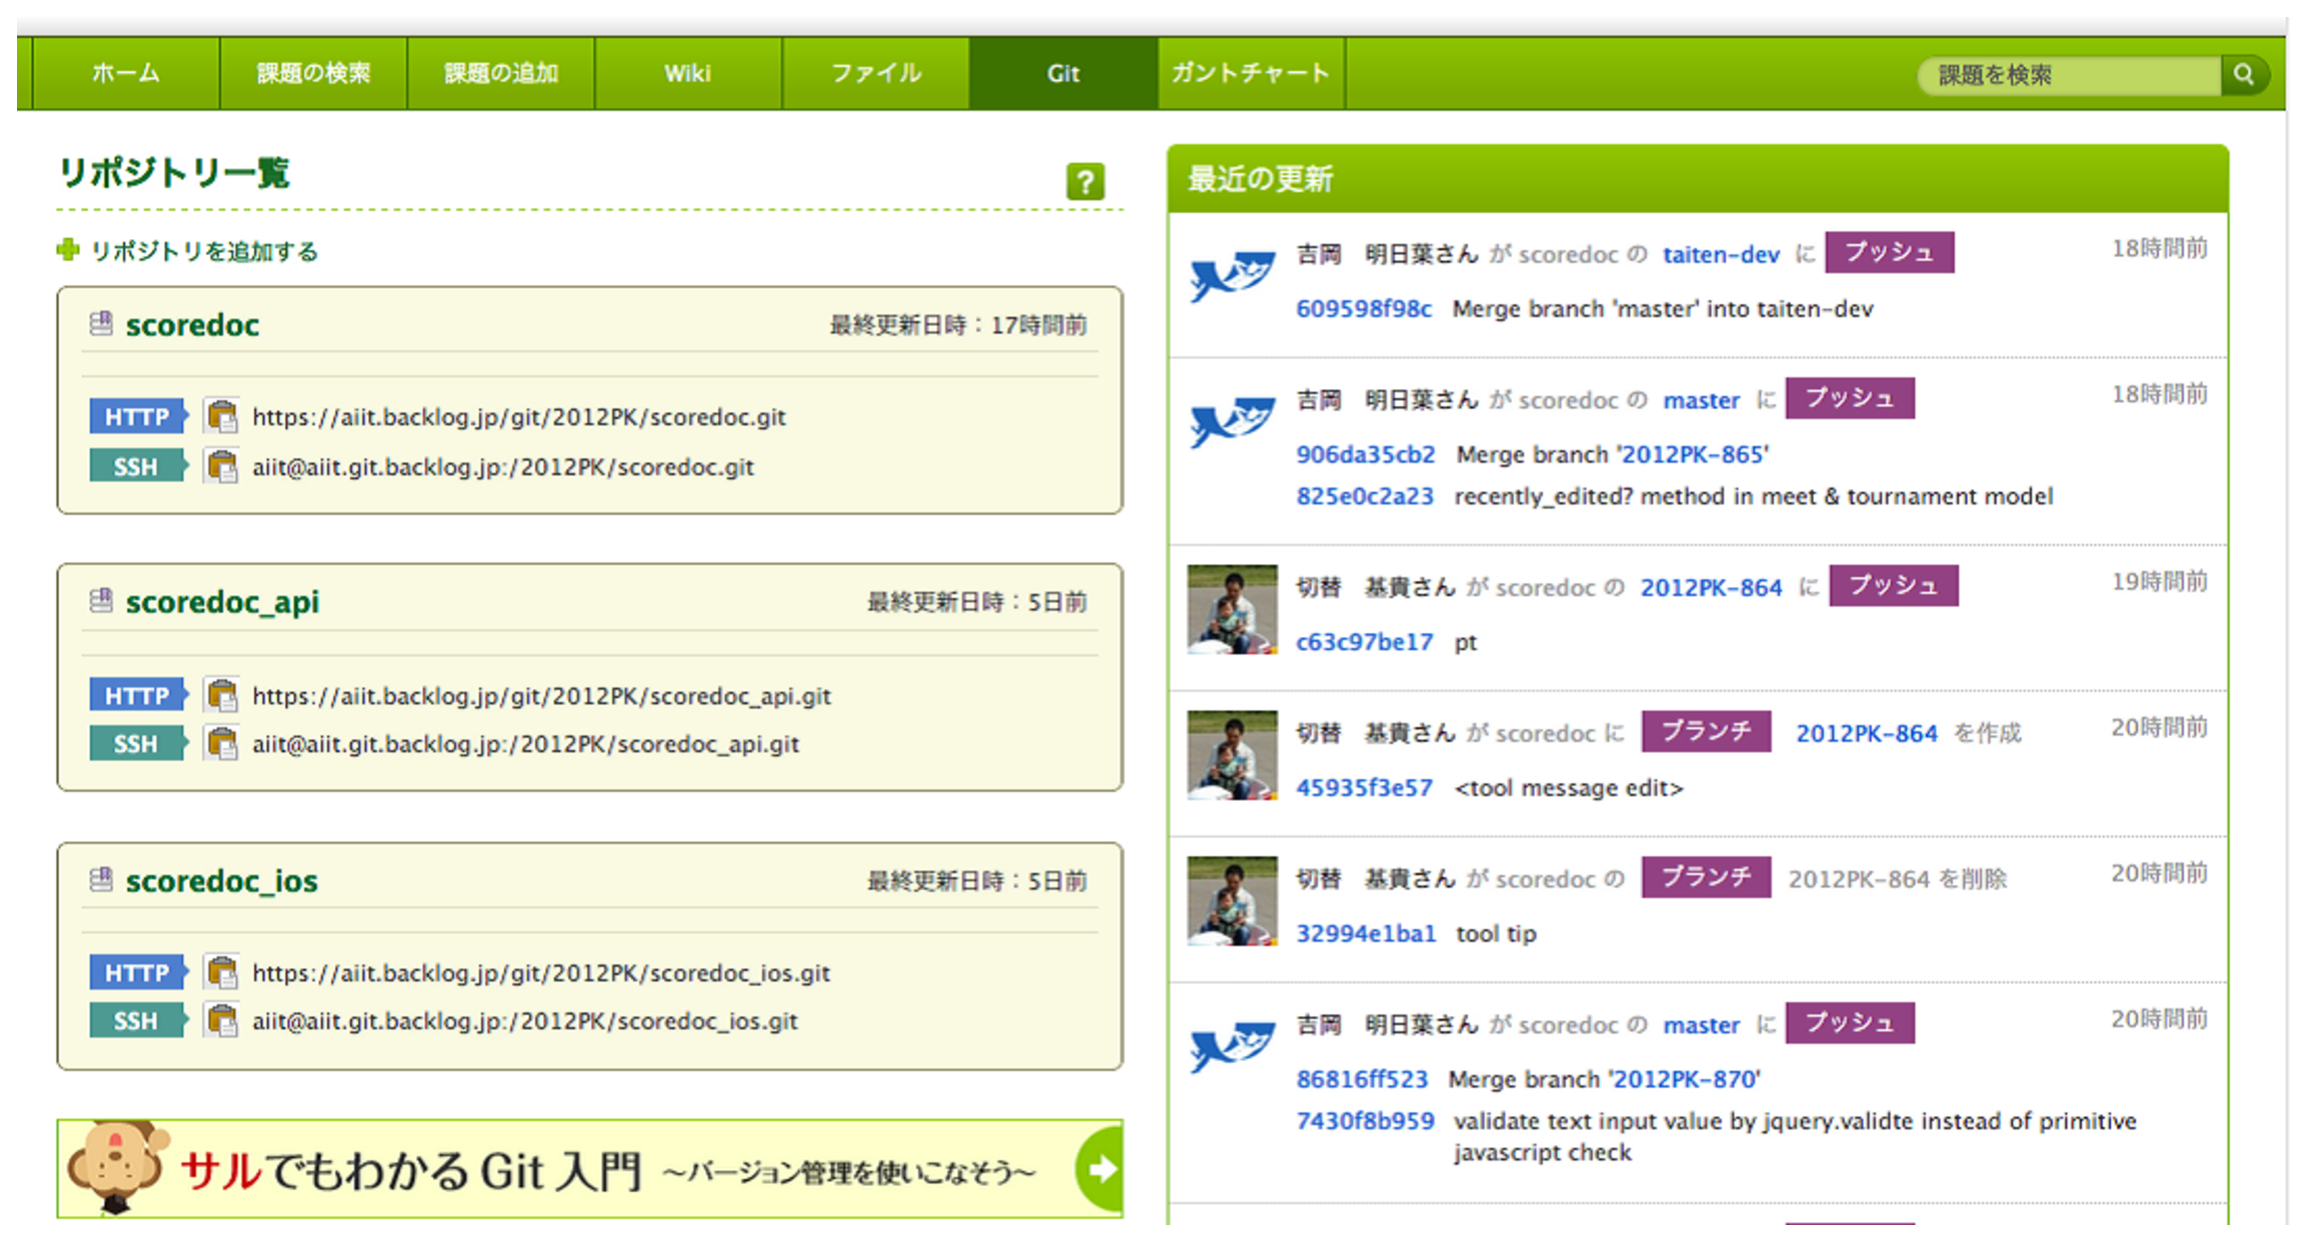
\includegraphics[width=7.5cm]{./figure/Git.eps}
\caption{Gitによるソースコード管理}
\label{fig:Git}
\end{figure}

\begin{figure}[t]
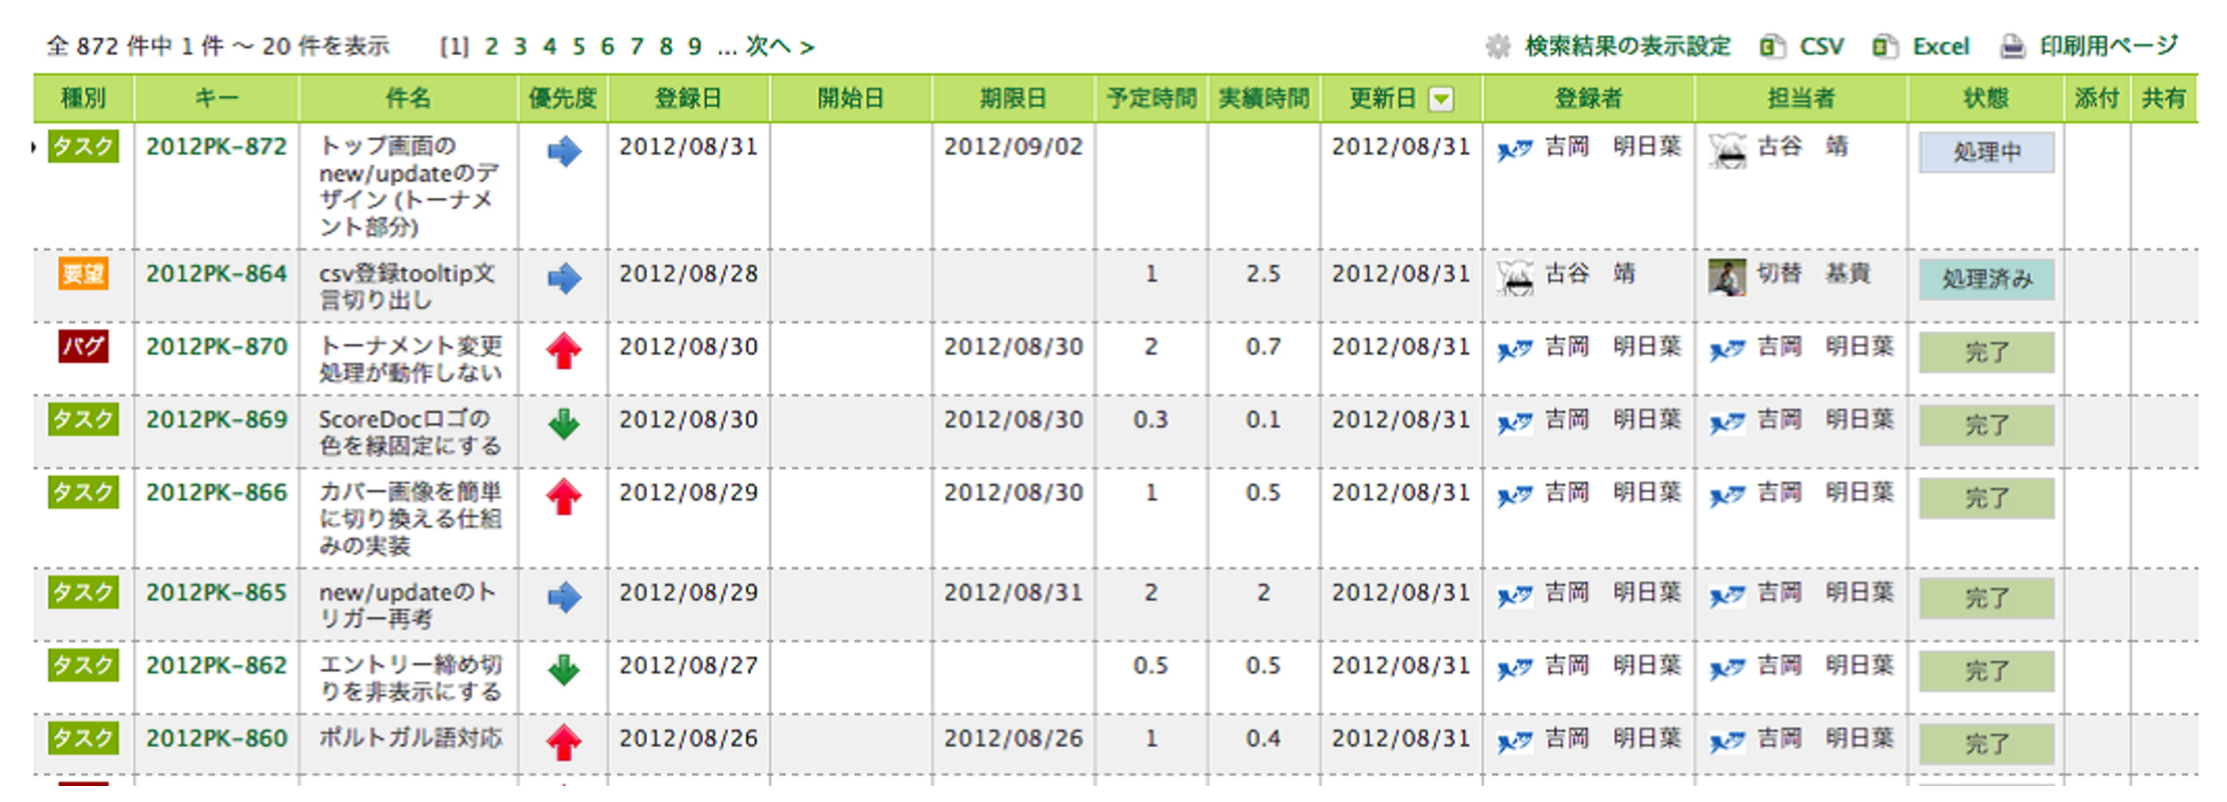
\includegraphics[width=7.5cm]{./figure/Issue.eps}
\caption{課題の管理画面}
\label{fig:Issue}
\end{figure}

\begin{figure}[t]
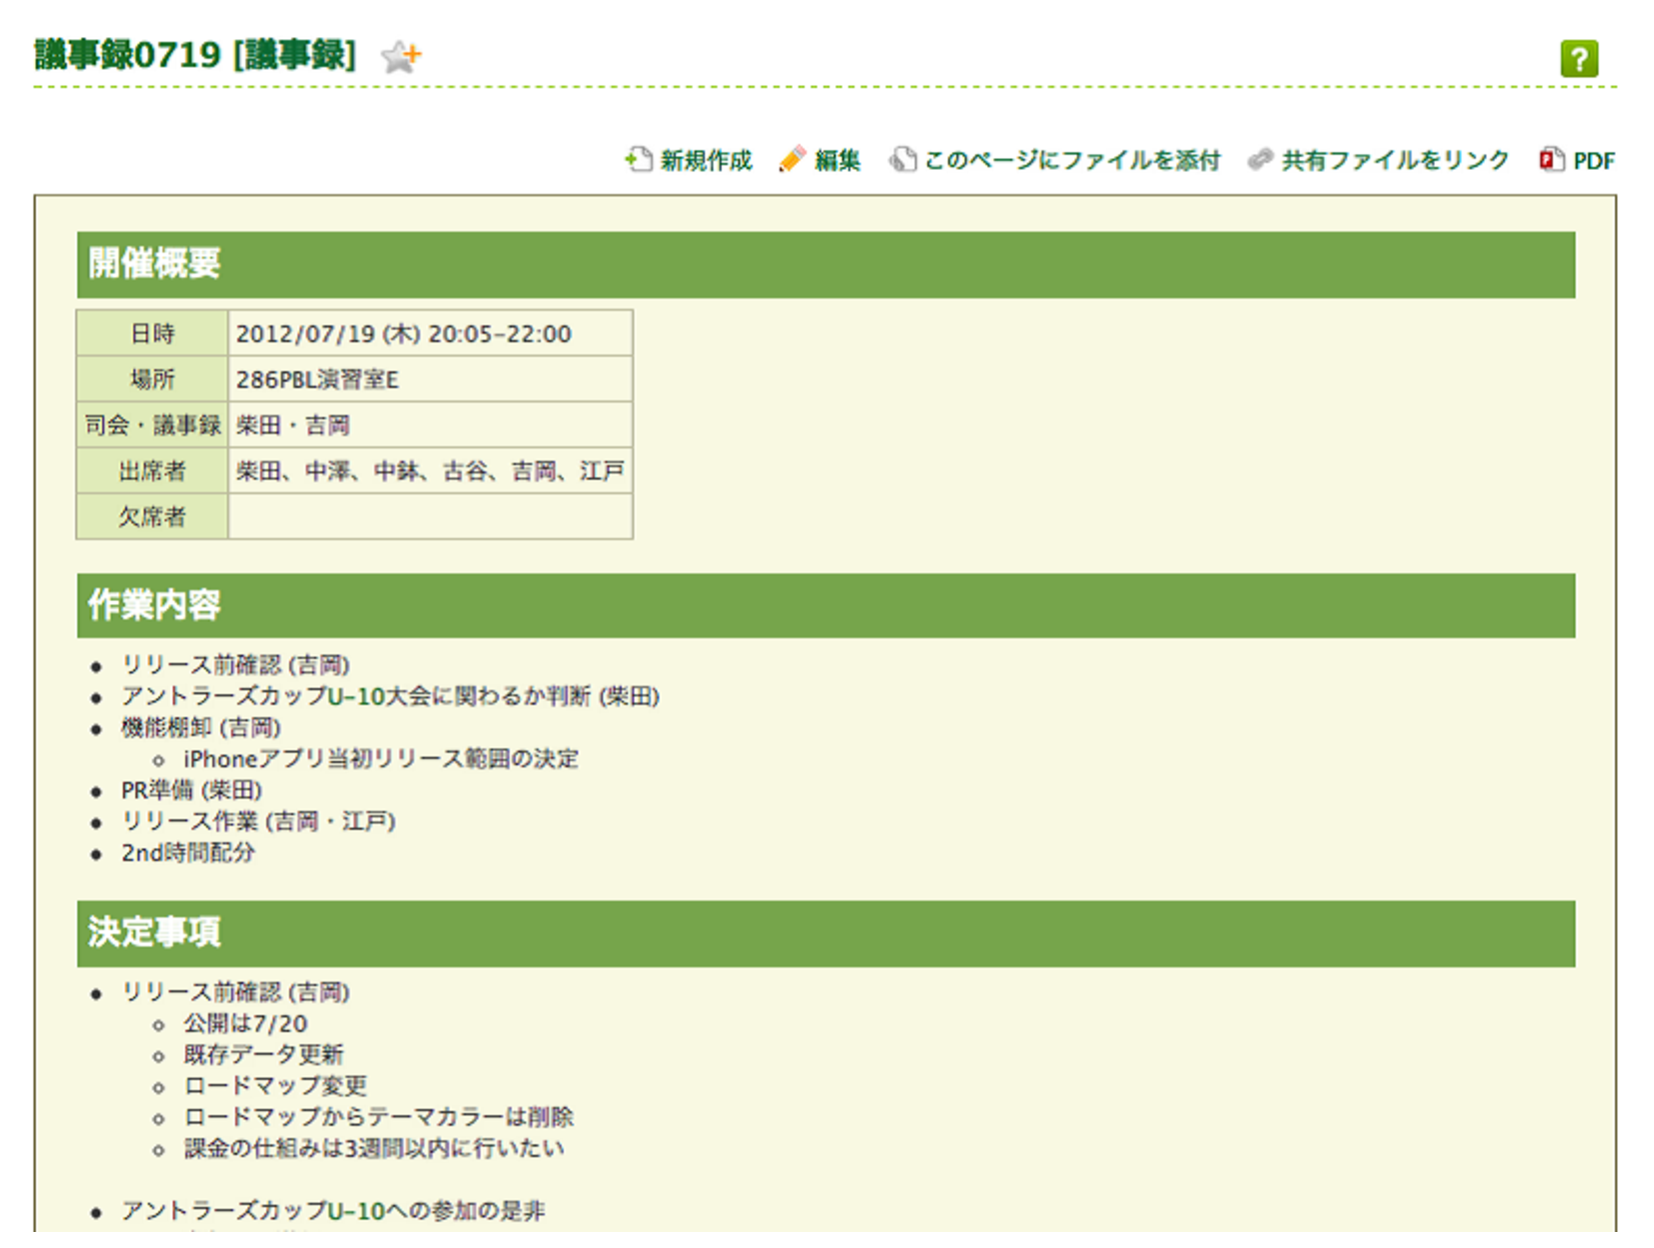
\includegraphics[width=7.5cm]{./figure/Wiki1.eps}
\caption{Wikiによる議事録の作成}
\label{fig:Wiki1}
\end{figure}

% \begin{figure}[tb]
% 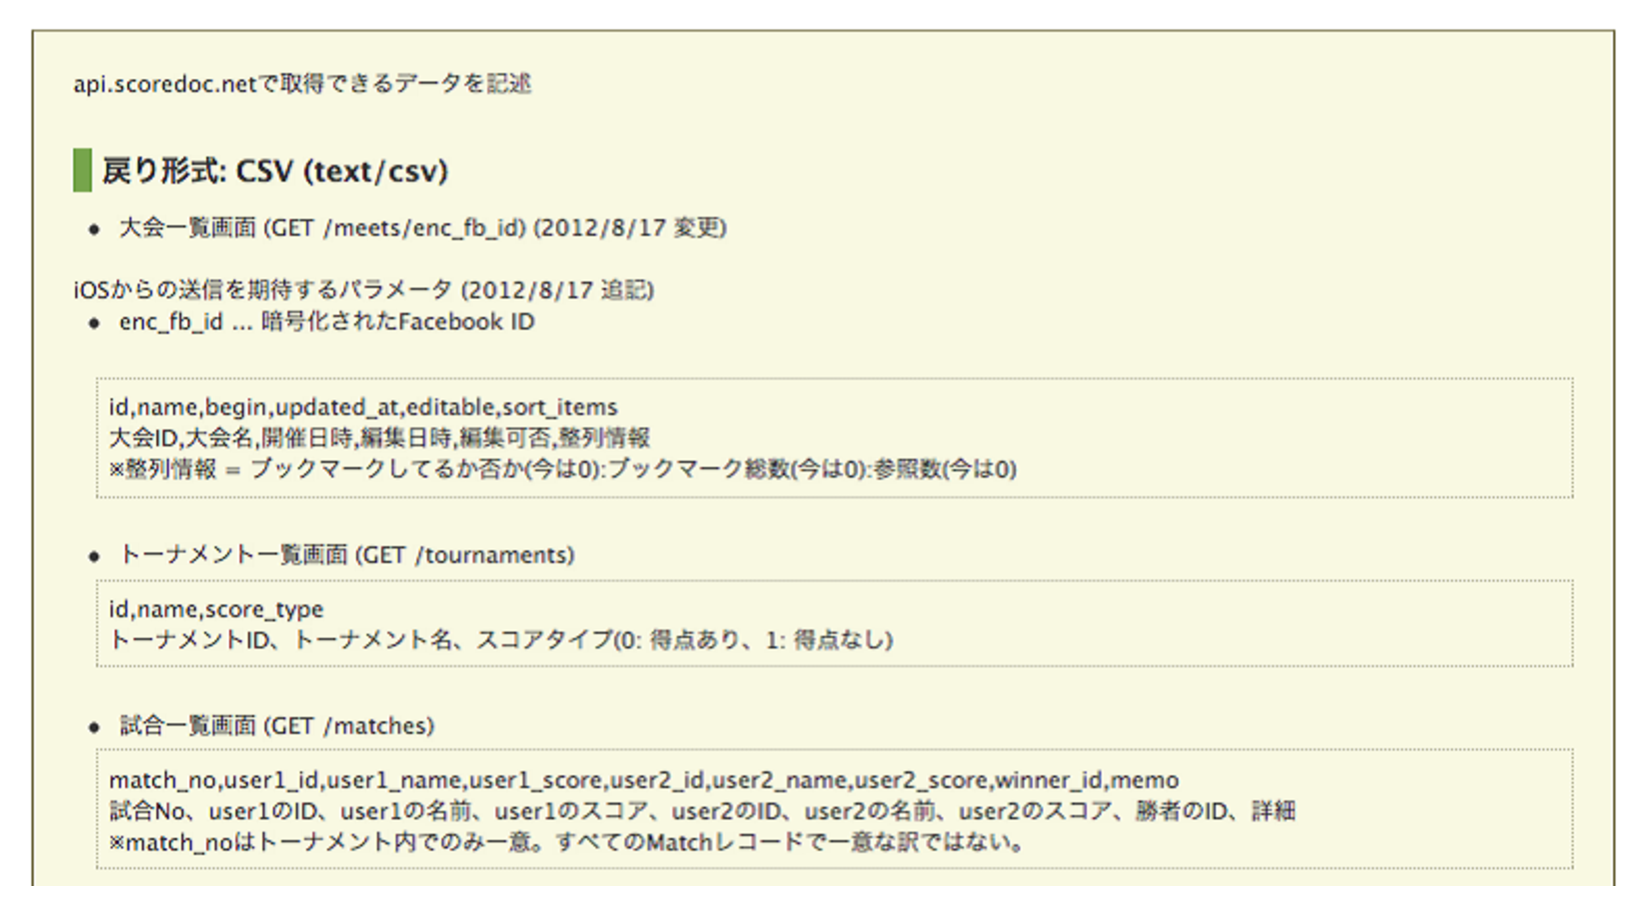
\includegraphics[width=7.5cm]{./figure/Wiki2.eps}
% \caption{Wikiの利用例}
% \label{fig:Wiki2}
% \end{figure}

\end{document}
